\documentclass[acmsmall,review,screen]{acmart}

\settopmatter{printfolios=true,printccs=true,printacmref=true}

\let\showappendix\relax
%% comment out to hide appendix + refs

\overfullrule=3mm
\citestyle{acmauthoryear}
%\setcitestyle{round}

\usepackage{multirow}

\usepackage{alltt}
% \usepackage{amssymb}
\usepackage{calc}
\usepackage[noabbrev]{cleveref}
\usepackage{colortbl}
\usepackage{listings}
\usepackage{mathpartir}
\usepackage{graphicx}
\usepackage{pifont}
\usepackage{subcaption}
\usepackage{tikz}
\usepackage{wrapfig}
\usepackage{xcolor}
\usetikzlibrary{arrows.meta}
\usetikzlibrary{positioning}
\usetikzlibrary{shapes.geometric}

\usepackage{moreverb}

%%%%%%%%%%%%%%%%%%%%%%%%%%%%%%%%%%%%%%%%%%%%%%%%%%%%%%%%%%%%%%%%%%%%%%%%%%%%%%%%%%%%%%%%%%%%
%%%%%%%%%%%%%%%%%%%%%%%%%%%%%%%%%%%%%%%%%%%%%%%%%%%%%%%%%%%%%%%%%%%%%%%%%%%%%%%%%%%%%%%%%%%%
%%%%%%%%%%%%%%%%%%%%%%%%%%%%%%           PREAMBLE       %%%%%%%%%%%%%%%%%%%%%%%%%%%%%%%%%%%% 
%%%%%%%%%%%%%%%%%%%%%%%%%%%%%%%%%%%%%%%%%%%%%%%%%%%%%%%%%%%%%%%%%%%%%%%%%%%%%%%%%%%%%%%%%%%%
%%%%%%%%%%%%%%%%%%%%%%%%%%%%%%%%%%%%%%%%%%%%%%%%%%%%%%%%%%%%%%%%%%%%%%%%%%%%%%%%%%%%%%%%%%%%

\usepackage{tcolorbox}
\usepackage{siunitx}

%%%%%%%%%%%%%%%%%%%%%%%%%%%%%%%%%%%%%%%%%%%%%%%%%%%%%%%%%%%%%%%%%%%%%%%%%%%%%%%%%%%%%%%%%%%%
%%%%%%%%%%%%%%%%%%%%%%%%%%%%%%%%%%%%%%%%%%%%%%%%%%%%%%%%%%%%%%%%%%%%%%%%%%%%%%%%%%%%%%%%%%%%
%%%%%%%%%%%%%%%%%%%%%%%%%%%%%%%%%%%%%%%%%%%%%%%%%%%%%%%%%%%%%%%%%%%%%%%%%%%%%%%%%%%%%%%%%%%%

\newcommand{\set}[1]{\ensuremath{\bar{#1}}}

\newcommand{\size}[1]{\ensuremath{\mid #1 \mid}}

\newcommand{\setsize}[1]{\left|#1\right|}



%% %%%%%%%%%%%%%%%%%%%%%%%%%%%%%%%%%%%%%%%%%%%%%%%%%%%%%%%%%%%%%%%%%%%%%%%%%%%%%
%% for leaving margin notes in the paper write
%% \yourinitials{...} 

\def\notes#1{\expandafter\def\csname#1\endcsname##1{\marginpar{\textcolor{red}{\raggedright\tiny $\bullet$ #1 says: ##1}}}}
\notes{mf}
\notes{cd}
\notes{bg}


%% %%%%%%%%%%%%%%%%%%%%%%%%%%%%%%%%%%%%%%%%%%%%%%%%%%%%%%%%%%%%%%%%%%%%%%%%%%%%%

%% strategies

\newcommand{\boundary}{boundary}
\newcommand{\feat}{\boundary}
\newcommand{\statistical}{statistical}

\newcommand{\sfont}[1]{\textit{#1}}

\newcommand{\featkw}{\sfont{\boundary}}

\newcommand{\statkw}{\sfont{\statistical}}

\newcommand{\totalkw}{\sfont{total}}

\newcommand{\selfkw}{\sfont{self}}

\newcommand{\stat}[1]{\sfont{\statkw(#1)}}

\newcommand{\statself}{\sfont{\stat{\selfkw}}}
\newcommand{\stattotal}{\sfont{\stat{\totalkw}}}

\newcommand{\optkw}{\sfont{optimistic}}

\newcommand{\conkw}{\sfont{conservative}}

\newcommand{\costkw}{\sfont{cost\textsf{-}aware}}

\newcommand{\confkw}{\sfont{configuration\textsf{-}aware}}

\newcommand{\randkw}{\sfont{null}}

\newcommand{\togglekw}{\sfont{toggling}}

\newcommand{\agnostickw}{\sfont{profiler\textsf{-}agnostic}}

\newcommand{\strategy}[2]{#1~#2}

\newcommand{\strategyext}[3]{#1~\strategy{#2}{#3}}


\newcommand{\featopt}{\strategy{\featkw}{\optkw}}
\newcommand{\statselfopt}{\strategy{\statself}{\optkw}}
\newcommand{\stattotalopt}{\strategy{\stattotal}{\optkw}}

\newcommand{\featcon}{\strategy{\featkw}{\conkw}}
\newcommand{\statselfcon}{\strategy{\statself}{\conkw}}
\newcommand{\stattotalcon}{\strategy{\stattotal}{\conkw}}

\def\costoptkw{\strategy{\costkw}{\optkw}}

\newcommand{\featcostopt}{\strategyext{\featkw}{\costkw}{\optkw}}
\newcommand{\statselfcostopt}{\strategyext{\statself}{\costkw}{\optkw}}
\newcommand{\stattotalcostopt}{\strategyext{\stattotal}{\costkw}{\optkw}}

\def\costconkw{\strategy{\costkw}{\conkw}}

\newcommand{\featcostcon}{\strategyext{\featkw}{\costkw}{\conkw}}
\newcommand{\statselfcostcon}{\strategyext{\statself}{\costkw}{\conkw}}
\newcommand{\stattotalcostcon}{\strategyext{\stattotal}{\costkw}{\conkw}}

\newcommand{\featconf}{\strategy{\featkw}{\confkw}}
\newcommand{\statselfconf}{\strategy{\statself}{\confkw}}
\newcommand{\stattotalconf}{\strategy{\stattotal}{\confkw}}

\newcommand{\randomopt}{\strategy{\randkw}{\optkw}}
\newcommand{\randomcon}{\strategy{\randkw}{\conkw}}

\newcommand{\toggle}{\togglekw}

%% types

\newcommand{\type}{\ensuremath{t}}

\newcommand{\deep}{\ensuremath{deep}}

\newcommand{\shallow}{\ensuremath{shallow}}


%% program, components, strategy

\newcommand{\program}{\ensuremath{P}}


\newcommand{\component}{\ensuremath{c}}

\newcommand{\strategyvar}{\ensuremath{S}}


%% lattice

\newcommand{\latticeL}{\mathcal{L}}

\newcommand{\lattice}[1]{\ensuremath{\latticeL\llbracket#1\rrbracket}}

\newcommand{\standardlattice}{\lattice{\system}{\kmap}}

\newcommand{\conf}{\ensuremath{k}}

\newcommand{\metric}{\ensuremath{\leq_{\latticeL}^{X}}}


\newcommand{\modem}{\ensuremath{M}}
\newcommand{\mode}[1]{\ensuremath{\modem\llbracket#1\rrbracket}}

\newcommand{\orderkw}{\ensuremath{<}} 
\newcommand{\ordered}[2]{\ensuremath{#1 \orderkw #2}}

\newcommand{\orderqkw}{\ensuremath{\leqslant}} 
\newcommand{\orderqed}[2]{\ensuremath{#1 \orderqkw #2}}

%% performance


\newcommand{\slowdownkw}{\ensuremath{slowdown}}
\newcommand{\slowdown}[2]{\ensuremath{\slowdownkw(#1,#2)}}

\newcommand{\takikawa}{\ensuremath{T}}

\newcommand{\pct}[1]{\SI{#1}{\percent}}

\begin{document}

\title{How Profilers Can Help Navigate Type Migration}

\author{Ben Greenman}
\orcid{0000-0001-7078-9287}
\affiliation{%
  \institution{PLT @ Brown University}
  \city{Providence}
  \state{Rhode Island}
  \country{USA}
}
\email{benjaminlgreenman@gmail.com}

\author{Matthias Felleisen}
\orcid{0000-0001-6678-1004}
\affiliation{%
  \institution{PLT @ Northeastern University}
  \city{Boston}
  \state{Massachusetts}
  \country{USA}
}
\email{matthias@ccs.neu.edu}

\author{Christos Dimoulas}
\orcid{0000-0002-9338-7034}
\affiliation{%
  \institution{PLT @ Northwestern University}
  \city{Evanston}
  \state{Illinois}
  \country{USA}
}
\email{chrdimo@northwestern.edu}

%\renewcommand{\shortauthors}{...}

%%
%% The abstract is a short summary of the work to be presented in the
%% article.
%% -----------------------------------------------------------------------------

\begin{abstract}
  Sound migratory typing envisions a safe and smooth refactoring of
  untyped code bases to typed ones.  However, the cost of enforcing safety
  with run-time checks is often prohibitively high, thus performance
  regressions are a likely occurrence.  Additional types can often
  recover performance, but choosing the right components to type is difficult
  because of the exponential size of the migratory typing lattice. In
  principal though, migration could be guided by off-the-shelf
  profiling tools.  To examine this
  hypothesis, this paper  follows the rational programmer method and
  reports on the results of an experiment on tens of thousands of
  performance-debugging scenarios via seventeen strategies for
  turning profiler output into an actionable next step.  The most
  effective strategy is the use of deep types to eliminate the most
  costly boundaries between typed and untyped components; this strategy
  succeeds in more than 50\% of scenarios if two performance
  degradations are tolerable along the way.
\end{abstract}
%%
%% The code below is generated by the tool at http://dl.acm.org/ccs.cfm.
%% Please copy and paste the code instead of the example below.

\begin{CCSXML}
<ccs2012>
<concept>
<concept_id>10011007.10011006.10011039.10011311</concept_id>
<concept_desc>Software and its engineering~Semantics</concept_desc>
<concept_significance>500</concept_significance>
</concept>
<concept>
<concept_id>10011007.10011006.10011008.10011024.10011032</concept_id>
<concept_desc>Software and its engineering~Constraints</concept_desc>
<concept_significance>100</concept_significance>
</concept>
<concept>
<concept_id>10011007.10011006.10011008.10011009.10011012</concept_id>
<concept_desc>Software and its engineering~Functional languages</concept_desc>
<concept_significance>100</concept_significance>
</concept>
</ccs2012>
\end{CCSXML}

\ccsdesc[500]{Software and its engineering~Semantics}
\ccsdesc[100]{Software and its engineering~Constraints}
\ccsdesc[100]{Software and its engineering~Functional languages}

\newcommand{\ifappendix}[2]{\ifdef{\showappendix}{#1}{#2}}
\newcommand{\code}[1]{\texttt{#1}}
\newcommand{\cmod}[1]{\parbox[c][1.4ex]{2em}{\code{#1}}}
\newcommand{\stdrkt}{\code{v8.6.0.2 [cs]}}
\newcommand{\bmname}[1]{\textsf{#1}}
\newcommand{\totalnumconfigs}{116,154}
\newcommand{\totalnummeasurements}{1277694}
%% 2023-03-22 bg: configs + runs ignoring quadT
\newcommand{\machinename}[1]{\texttt{#1}}
\newcommand{\commitname}[2]{\texttt{#1}}
\newcommand{\gcell}[1]{\cellcolor{green!20}#1}
\newcommand{\wcell}[1]{\cellcolor{black!05}#1}
\newcommand{\ycell}[1]{\cellcolor{yellow!18}#1}
\newcommand{\ocell}[1]{\cellcolor{orange!29}#1}
\newcommand{\rcell}[1]{\cellcolor{red!30}#1}
\newcommand{\tcell}[1]{\cellcolor{black!10}#1}

\keywords{gradual typing, migratory typing, rational programmer, profiling}

\maketitle

%% -----------------------------------------------------------------------------

\section{Type Migration as a Navigation Problem}
\label{sec:intro}
%% -----------------------------------------------------------------------------

Sound migratory typing promises a safe and smooth refactoring path from an
untyped code base to a typed one~\cite{tf-dls-2006, tfffgksst-snapl-2017}. It
realizes the safe part with the compilation of types to run-time checks that
guarantee type-level integrity of each mixed-typed program configuration.
Unfortunately, these run-time checks impose a large performance
overhead~\cite{gtnffvf-jfp-2019}, making the path anything but smooth.
This problem is particularly stringent for deep run-time
checks~\cite{tf-dls-2006, st-sfp-2006}, but it also applies to shallow run-time
checking~\cite{gm-pepm-2018}.
While improvements to deep and shallow can reduce the severity of the
problem, in particular JIT technology for
shallow~\cite{rmhn-ecoop-2019,vsc-dls-2019},
the core issue remains---some configurations need more expensive checks than
others.

\citet{g-thesis-2020,g-deep-shallow} presents evidence that deep and shallow
checks actually come with complementary strengths and weaknesses. Deep checks
impose a steep cost at boundaries between typed and untyped code, yet as
the addition of types eliminates such boundaries, they
enable type-driven optimizations that can offset some of the
cost~\cite{s-northeastern-2015}---and sometimes all of it.
By contrast, shallow checks impose a low cost at boundaries, but the addition
of types almost always increases the overall number of checks.
Hence, Greenman argues that developers should, in
principle, be able to mix and match deep and shallow checking to get the
best-possible type checking benefits with a tolerable performance penalty.
Initial empirical data is promising: with the right mixture of checks,
it is possible to avoid order-of-magnitude slowdowns that come from either
deep or shallow checks alone.
Finding a ``right'' mixture, however, presents a challenge because there
are exponentially many possibilities to choose from.
Whereas in a purely deep (or shallow) checking scheme, developers have
$2^N$ configurations to choose from, with deep and shallow combined
there are $3^N$ possibilities because each of the $N$ components in
the program can be untyped, deep-typed, or shallow-typed.

The large search space raises the following question:
\begin{quote} \em
 How to navigate the $3^N$ migration lattice of a code base from a
  configuration with unacceptable performance to one with acceptable
  performance?
\end{quote}
Since this is a performance problem, a plausible answer is to use profiling tools.
%% ... readymade ... off-the-cuff ... glib
But, this conventional response merely refines the above question in two
ways, namely:
\begin{itemize} \item[] \begin{itemize}\em
\item How to use feedback from various profiling tools to choose a next step; and
\item Whether a sequence of choices leads to a configuration with
  acceptable performance.
\end{itemize} \end{itemize}

Such questions call for an empirical investigation.
A user study is a viable way forward, but recruiting a large number
of people to debug problems in unfamiliar code is costly and introduces
confounding factors.
Until recently, however, there was no other way to proceed systematically.
Instead, this paper reports on the results of a \emph{rational programmer}
experiment~\cite{lksfd-popl-2020,lgfd-icfp-2021,lgfd-icfp-2023}.
The rational programmer method employs algorithmic abstractions (\emph{strategies})
that are inspired by methods that actual humans can follow and that reify a
falsifiable hypothesis about one way of using profiling tools and
interpreting their feedback.
Because the strategies are algorithms, it is straightforward to apply them
to thousands of debugging scenarios and test whether they improve performance.
In sum, the rational programmer experiment enables a systematic comparison
of different ways that human developers\footnote{To distinguish
between humans and the rational programmer, the 
paper exclusively uses ``developer'' for human coders.} might interpret profiler feedback.
The winning strategies merit further study, while the losing ones can be
set aside.

In short, this paper makes three contributions:
\begin{itemize}

\item At the technical level, the rational programmer experiment presents
  the most comprehensive and systematic examination of type migration
    paths to date.    As such it goes far beyond ~\citet{g-deep-shallow}'s 
    prior work.  The experiment evaluates 17 different strategies for
    interpreting profiling output on  more than one hundred thousand scenarios using the GTP
    benchmarks~\cite{g-rep-2023}. It yields
     5GB of performance and profiling data, which
    is available online~\cite{gdf-artifact-2023}.

\item At the object level, the results of the rational programmer
    experiment provide guidance to developers about how to best use feedback
    from profilers during type migration. The winning strategy
    identifies the most expensive boundary and migrates its components
    to use deep types.
    This result is a \emph{surprise} given~\citet{g-deep-shallow}'s
    preliminary data, which implies that combinations of shallow and
    deep types should lead to the lowests costs overall.

     \item[]\begin{itemize}
      \item
         Hence, the results also inform language designers about
         performance dividends from investing in combinations of deep and shallow types.
    \end{itemize}


\item At the meta level, this application of the rational programmer method to
 the performance problems of type migration provides evidence for its versatility
 as an instrument for studying language pragmatics.

\end{itemize}
The remainder of the paper is organized as follows.  \Cref{sec:seascape}
uses an example to explain the problem in concrete terms. \Cref{sec:ideas}
introduces the rational programmer method and shows how its use can systematically
evaluate the effectiveness of a performance-debugging strategy.
\Cref{sec:experiment} translates these ideas to a
large-scale quantitative experiment.
\Cref{sec:results} presents the data from the experiment, which
explores scenarios at a module-level granularity in Typed Racket.
\Cref{sec:discussion} extracts lessons for developers and researchers.
\Cref{sec:related} places this work in the context of prior research.
\Cref{sec:conclusion} puts this work in perspective with respect to future
research.

\section{Navigating the Deeps and Shallows by Profiling}
\label{sec:seascape}
%% -----------------------------------------------------------------------------

Over the years, developers have created many large systems in untyped languages.
In the meantime, language implementors have created gradually typed siblings of
these languages.  Since developers tend to enjoy the benefits of type-based IDE
support and a blessing from the type checker, they are likely to add new
components in the typed sibling language. Alternatively, when a developer must
debug an untyped component, it takes a large mental effort
to reconstruct the informal types of fields, functions, and methods, and to make
this effort pay off, it is best to turn the informal types into formal
annotations. In either case, the result is a mixed-typed software system
with components that have types and parts that do not.

In a sound gradual language, the enforcement of types inflicts a performance penalty.
Among the several enforcement approaches that do not limit
 expressiveness~\cite{type-untyped},\footnote{Nom~\cite{mt-oopsla-2017} and Static
Python~\cite{lgmvpk-pj-2023} have low-cost but restrictive
checks.} the two leading ones are deep and shallow types:
\begin{itemize}
  \item
    Deep types use higher-order contracts to monitor the
    boundaries between typed and untyped
    components~\cite{ff-icfp-2002,tf-dls-2006,st-sfp-2006}.  Higher-order
    contracts impose many kinds of performance penalties: they traverse
    compound values; they wrap higher-order values with proxies to delay
    checks; and they raise memory consumption due to the proxies'
    allocation.  If there are few boundaries, however, then deep types
    impose few costs and type-driven optimizations may exceed the
    performance of the untyped code base~\cite{gtnffvf-jfp-2019}.

  \item
    Shallow types do not explicitly enforce types at boundaries but
    delegate checking to tag-level assertions injected at
    compile-time at strategic places in typed components. Shallow's assertions
    ask simple questions (is this a list?) and never allocate
    proxies~\cite{vss-popl-2017, vksb-dls-2014}.  Each check is
    inexpensive, but the lack of proxies blurs the boundary between typed and
    untyped components and leads to a conservatively high number of checks.
    Suppose a typed function expects a callback.  To account for the case
    that the callback is supplied by an untyped component, every call needs a
    result check around it to ensure soundness---even if most calls are
    safe.  In general, the addition of more shallow types can lead to more
    checks.

\end{itemize}
In either case, the performance penalty can become too high.
If so, the developer faces a performance-debugging scenario.

To make these ideas concrete, consider the \bmname{fsm} program from the GTP benchmark
suite~\cite{gtnffvf-jfp-2019,g-rep-2023}. The program is the creation of \citet{fsm},
economists interested in simulating an economy of agents with deterministic
strategies. \Cref{f:fsm-code:a} shows the outline of the four-module
program: \code{auto} implements state machines; \code{pop} coordinates among
machines; \code{main} drives the simulation;
%% and permits users to set a number of simulation parameters
and \code{util} provides helper functions.  Focusing on
just the modules of this program suffices because the migration granularity
in Typed Racket is by module (each module can be typed or untyped).

%% -----------------------------------------------------------------------------
%% fsm next steps:
%% 1100 => 2.87x
%% 2100 => 9.04x
%% 2200 => 9.06x
%% 1200 => 2.88x

\begin{figure}[htb]\centering
  %% profiler output: data/example-output-fsm/*

  \begin{subfigure}[t]{\columnwidth}\centering
    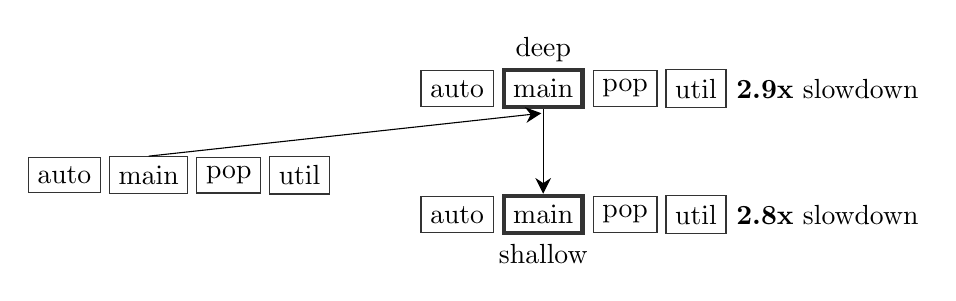
\begin{tikzpicture}
      \node (1) [draw=black!80] {\cmod{util}};
      \node (1c) [draw=black!80,left=of 1.west,xshift=9mm] {\cmod{pop}};
      \node (1b) [draw=black!80,left=of 1c.west,xshift=9mm] {\cmod{main}};
      \node (1a) [draw=black!80,left=of 1b.west,xshift=9mm] {\cmod{auto}};
%      \node (0) [above of=1a,yshift=-2mm] {Program: \bmname{fsm}};

      \node (2) [above of=1,yshift=1mm,xshift=2cm,draw=black!80] {\cmod{auto}};
      \node (2a) [draw=black!80,line width=0.6mm,right=of 2.east,xshift=-9mm] {\cmod{main}};
      \node (2tgt) [below of=2a,yshift=7mm,xshift=1mm] {};
      \node (2b) [draw=black!80,right=of 2a.east,xshift=-9mm] {\cmod{pop}};
      \node (2c) [draw=black!80,right=of 2b.east,xshift=-9mm] {\cmod{util}};
      \node (22) [right=of 2c.east,xshift=-10mm] {\textbf{2.9x} slowdown};
%      \node (24) [above of = 22,yshift=-6mm] {Deep types};

      \node (3) [below of=2,yshift=-6mm,draw=black!80] {\cmod{auto}};
      \node (3a) [draw=black!80,line width=0.6mm,right=of 3.east,xshift=-9mm] {\cmod{main}};
      \node (3b) [draw=black!80,right=of 3a.east,xshift=-9mm] {\cmod{pop}};
      \node (3c) [draw=black!80,right=of 3b.east,xshift=-9mm] {\cmod{util}};
      \node (33) [right=of 3c.east,xshift=-10mm] {\textbf{2.8x} slowdown};
%      \node (34) [above of = 33,yshift=-6mm] {Shallow types};

      \node (dlbl) [above of=2a,yshift=-5mm] {deep};
      \node (slbl) [below of=3a,yshift=5mm] {shallow};

      \draw[-{Stealth[length=2mm,width=2mm]}] (1b.north) -- (2tgt);
      \draw[-{Stealth[length=2mm,width=2mm]}] (2a.south) -- (3a.north);

    \end{tikzpicture}

    \caption{Adding deep or shallow types to one \bmname{fsm} module degrades performance} \label{f:fsm-code:a}
  \end{subfigure}

  \bigskip

  \begin{subfigure}[t]{0.53\columnwidth}
%%-------------------------------------------------
%% [1] 1192(100.0%)   0(0.0%)  body of ....
%%                              body of ....
%%-------------------------------------------------
%%                              profile-thunk [5]
%% [6] 1192(100.0%)   0(0.0%)  ??? profile-lib
%%                              body of "main" [7]
%%                              t [8]
%%                              body of ....
%%-------------------------------------------------

    \footnotesize
    \begin{boxedverbatim}
  Total cpu time observed: 1192ms (out of 1236ms)
  Number of samples taken: 23 (once every 52ms)

=================================================
                              Caller
 Idx   Total       Self      Name+src
       ms(pct)     ms(pct)    Callee
=================================================
                              ??? [12]
                              evolve [17]
[17]  818(68.6%)    0(0.0%)  evolve main
                              evolve [17]
                              shuffle-vector [19]
                              death-birth [18]
                              ??? [20]
-------------------------------------------------
                              match-up* [22]
                              shuffle-vector [19]
[24]  152(12.7%)  152(12.7%) contract-wrapper
-------------------------------------------------
    \end{boxedverbatim}
    \caption{Statistical profiler output for the top-right variant} \label{f:fsm-code:statistical}
  \end{subfigure}~\begin{subfigure}[t]{0.44\columnwidth}
    \footnotesize
    \begin{boxedverbatim}
cpu time: 984 real time: 984 gc time: 155
Running time is 18.17% contracts
253/1390 ms

(interface:death-birth pop main)
  142 ms
  (->* ((cons/c (vectorof automaton?)
                (vectorof automaton?))
        any/c)
       (#:random any/c)
       (cons/c (vectorof automaton?)
               (vectorof automaton?)))
(interface:match-up* pop main)
  81.5 ms
  (-> ....)
(interface:population-payoffs pop main)
  29 ms
  (-> ....)


    \end{boxedverbatim}
    \caption{Boundary profiler output for the same variant} \label{f:fsm-code:boundary}
  \end{subfigure}

  \caption{Profiling during type migration} \label{f:fsm-code}
  \Description{Profiling during type migration} 
\end{figure}
%% -----------------------------------------------------------------------------

The variant of \bmname{fsm} on the left of figure~\ref{f:fsm-code:a} is untyped.
If a developer adds deep types to the \code{main} module, performance is
significantly degraded. The mixed-typed variant runs almost three times
($3x$) slower than the untyped one.  Switching to shallow types is a one-line
change to the module language, but does not remedy the situation.
At this point, the question is how to recover the performance of the untyped
variant. Each results in different kind of costs  
\begin{itemize} \item[] \begin{itemize}
  \item
One option is to roll back the addition of types.
  \item
For developers who prefer typed code and dislike undoing the effort of
adding types, a second option is to add
(deep or shallow) types to a random module connected to \code{main}---following a
``hunch'' like developers sometimes do---but doing so can easily make things
worse. For example, if the choice were the \code{auto} module with shallow
types, then performance would degrade further (a 9x slowdown, to be
precise).
  \item
If the developer adds deep types to every module, then \bmname{fsm}
has no type boundaries and gets the full benefit of optimizations. Performance
improves over the untyped variant.
However, such a choice
represents a heavy migration effort, which a developer who simply
wishes to fix \code{main} and deploy again may be reluctant to invest.
\end{itemize} \end{itemize}
None of these options are compelling.
Informed feedback is clearly needed for a solution that recovers performance
with a reasonable effort and without discarding types.

The natural choice is to reach for a
profiling tool to determine the source of the slowdown.
Racket fortunately comes with two such tools: 
\begin{itemize} \item[] \begin{itemize}

\item a traditional \emph{statistical profiler}, which identifies the time spent
 in applications; and

\item a \emph{boundary profiler}, which  attributes the cost of types-as-contracts to
 specific module boundaries~\cite{astavf-feature-prf, staaf-feature-prf}.

\end{itemize} \end{itemize}
Both tools are potentially useful and potentially limited due to the mechanics
of deep and shallow types. Specifically, the contract-based enforcement of
deep types should be a good match for the boundary profiler but not
for the statistical profiler. In contrast, shallow checks
should favor the statistical but not the boundary profiler.
For example, the function below averages a list of numbers.
While the total run-time costs of deep or shallow types are comparable
for this function, those costs arise in different ways:

\begin{verbatim}
  (: avg (-> [Listof Real] Real))         ;; deep: enforce type as a contract
  (define (avg l) (/ (sum l) (length l))) ;; shallow: rewrite code with checks
\end{verbatim}

\begin{itemize}
  \item
    With deep types, the function gets wrapped in a proxy at the boundary
    between \code{avg} and its untyped clients.
    The proxy checks that clients send only lists that contain
    only real numbers.
    The \emph{boundary profiler} is well-suited to
    discover if these checks are expensive because it attributes costs
    directly to proxies.
    Conversely, the statistical profiler is less
    likely to be useful because it breaks down cost by application.
    It may, however, discover the costs indirectly if the proxy slows
    down calls to functions that, in turn, call \code{avg}.
  \item
    With shallow types, the compiler rewrites the body of \code{avg} to
    check that its clients send only lists. This check does not examine
    list elements, but the helper function \code{sum} will check elements
    as it accesses them.
    Because there are no contracts and explicit boundaries
    in the shallow version, only simple inlined checks, the
    boundary profiler cannot measure the cost of the types.
    The \emph{statistical profiler} is in a much better position to find
    costs because they arise from extra code in the function.
\end{itemize}

Back to \bmname{fsm}, 
the bottom half of \cref{f:fsm-code} shows the output of the statistical
profiler and the boundary profiler for the top-right variant in
\cref{f:fsm-code:a} where \code{main} has deep types.

\paragraph{Statistical profiler} \Cref{f:fsm-code:statistical} lists two
rows from the statistical profiler; the full output has 28 rows.  The
first row, labeled \code{[17]}, covers a large percentage (\code{68.6\%}) of the
total running time, and it refers to a function named \code{evolve}, which is
defined in the \code{main} module. The line suggests that calls from
\code{evolve} to other functions account for a high percentage of the total cost.
The second row, labeled \code{[24]}, says that a contract wrapper accounts for a
significant chunk (\code{12.7\%}) of the running time.  The caller of this
contract, from row \code{[19]} (not shown) is the function \code{shuffle-vector}
from the \code{pop} module.  Putting these clues together, the profiling output
indirectly points to the boundary between \code{main} and \code{pop} as a significant
contributor to the overall cost. 

This conclusion, however, is one of many that could be drawn from the full
statistical profiler output.  Functions from the \code{util} module also appears in the output,
and may be more of a performance problem that those from the \code{pop} module.  Equally
unclear is whether the column labeled \code{Total} is a better guide than
the column labeled \code{Self} or vice versa.  High
total times point to a context that dominates the expensive parts.  High self
times point to expensive parts, but these costs might be from the actual
computation rather than the overhead of type-checking.

\paragraph{Boundary profiler} \Cref{f:fsm-code:boundary} shows nearly-complete
output from the boundary profiler; only two contracts are omitted.  This
profiling output attributes \code{18.17\%} of the total running time to
contracts, specifically, to the contracts on the three functions whose names
begin with an \code{interface:} prefix.
This output indicates that proxies are
wrap untyped functions that flow into typed components. The modules involved are
\code{main} and \code{pop}.  Since \code{pop} is the untyped one, the hint is to
type it.

Adding types to \code{pop} does improve performance. Concretely, this variant
suffers from a 1.2x slowdown.  If this overhead is acceptable, the developer is
done; otherwise, the search must continue with another round of
profiling, searching, and typing.


\paragraph{Summary}

At first glance, the effort of eliminating a performance problem seems
straightforward. Several factors complicate the search. First, a
developer has two typing options not just one. Second, the output from
profiling tools is complex. Even for this small program, the statistical
profiler outputs 100 lines;
identifying the next step is hard. Finally, adding types to the
profiler-identified module may degrade the performance even more, in which case
the developer may wish to give up. In sum:

\begin{quote} \em
Navigating a migration lattice with
$3^N$ program configuration is a non-trivial effort, and developers deserve to
know how well profiling tools help with this effort.
\end{quote}


\section{A Rational Approach to Navigation}
\label{sec:ideas}
%% -----------------------------------------------------------------------------

When a performance-debugging scenario arises, the key question is \emph{how
to modify the program} to improve performance.
Profiling tools provide data, but there are many ways to interpret this data.
The rational programmer method proceeds by enumerating possible
interpretations and testing each one independently.

To begin, the type-migration lattice suggests two general ways to modify a
code base:
add types to an untyped component, or toggle the types of a typed one
from deep to shallow or vice versa.
The next question is which component to modify.
Since profiling tools identify parts of the code base that contribute to performance
degradation, the logical choice is to rank them using a relevant, deterministic
order and modify the highest-priority one.

Stepping back, these two insights on modifications and ordering suggest
an experiment to determine which combinations of profiling tool,
ordering, and modification strategy help developers make progress with
performance debugging.
To determine the best combination(s), developers must work through a
large and diverse set of performance-debugging scenarios.
The result should identify successful and unsuccessful strategies for ranking
profiler output and modifying code.
Of course, it is unrealistic to ask human developers to follow faithfully different
strategies through thousands
of scenarios. An alternative experimental method is needed.

The rational programmer provides a framework for conducting such
large-scale systematic examinations.
It is inspired by the well-established idea of rationality in
economics~\cite{mill1874essays, henrich2001search}.  In more detail, a
rational agent is a mathematical model of an economic actor. Essentially, it
abstracts an actual economic actor to an entity that, in any given
transaction-scenario, acts strategically to maximize some kind of benefit.
These agents are (typically) bounded rather than perfectly rational
to reflect the limitations of human beings and of available information;
they aim to \emph{satisfice}~\cite{hs:satisfice} their goal since
they cannot make maximally optimal choices.
Analogously, a rational programmer is a model of a developer who aims to
resolve problems with bounded resources.
Specifically, it is an algorithm that implements a developer's bounded
strategy for {satisficing} a goal, and thereby enables a large-scale
experiment.
Developers can use the outcomes of an experiment to decide whether
``rational'' behavior seems to pay off.
In other words, a rational programmer evaluation yields insights into the
pragmatic value of work strategies.

So far, the rational programmer has been used to evaluate
strategies for debugging logical mistakes.\footnote{Prior work
distinguishes between \emph{strategies} for interpreting data and
\emph{modes} of the rational programmer, which combine a strategy and other
parameters into an algorithm. Our experiment has only one parameter, the
strategy, and therefore the distinction between strategy and mode is
unimportant here.}
This paper presents the first application to a performance problem.

%% -----------------------------------------------------------------------------
\paragraph{Experiment Sketch.}
In the context of profiler-guided
type migration, a rational programmer consists of two interacting pieces.  The
first is strategy-agnostic; it consumes a program, measures its running time,
and if the performance is tolerable, stops. Otherwise, the program is a
performance-debugging scenario and the second,
strategy-specific piece comes into play. This second piece profiles the given program---using
the boundary profiler or the statistical profiler---and analyzes the
profiling information. Based on this analysis, it modifies the program
as described above.
This modified version is handed back
to the first piece of the rational programmer.

There are many strategies that might prove useful.
A successful strategy will tend to eliminate performance overhead,
though perhaps after a few incremental steps.
An unsuccessful strategy will either degrade performance, or fail
to reach a fast configuration.
Testing several strategies sheds light on their relative usefulness.
If one strategy succeeds where another fails, it has higher relative value.
Of course, the experiment may also reveal shortcomings of the profiling approach
altogether---which would demand additional research from tool creators.


\section{Experiment Design}
\label{sec:experiment}
%% -----------------------------------------------------------------------------

Turning the sketch from section~\ref{sec:ideas} into a large-scale
automated experiment requires formal descriptions for both the profiling
strategies of the rational programmer and the notion of debugging
scenario. As the preceding section discusses, given a scenario, a strategy
identifies the next migration step, which should yield either an acceptable
program or another performance-debugging scenario.  The preceding section
also implies that the migration step is one of three possibilities: (1)
to add types and to specify their enforcement regime (deep, shallow); (2)
to toggle from one regime to another; or (3) to fail to act. Hence it is
possible to specify strategies independently of the scenarios per se.
Equipped with formal descriptions, it is possible to turn the generic
research question of the introduction into questions with a quantitative
nature.

\Cref{subsec:strategies} presents the profiling strategies.
\Cref{subsec:lattice} characterizes performance-debugging
scenarios, which act as starting navigation points,
and how a type-based migration is a path
through a lattice of program configurations.
It also lays out the criteria for successes and failures for strategies.
Finally, \cref{subsec:questions} formalizes the precise experimental
questions and the experimental procedure that answers them.

%% -----------------------------------------------------------------------------

\subsection{The Rational Programmer Strategies}
\label{subsec:strategies}
%% -----------------------------------------------------------------------------
Every program \program{} is a collection of interacting components $\component$.
Some components have deep types, some have shallow ones, and some
are untyped. Independently of their types, a component $\component{}_1$, may
import another component $\component{}_2$, which establishes a \emph{boundary}
between them, across which they exchange values at run time. Depending on the
kind of types at the two sides of the boundary, a value exchange can trigger
run-time checks, which may degrade performance.

A profiling strategy should thus aim to eliminate the most costly
checks in a program. In formal terms, a profiling strategy is a
function that consumes a program \program{} and, after determining its
profile, returns a set of pairs $(\component{}, \type{})$. Here \type{} is
either \deep{} or \shallow{}. Each such pair prescribes a modification of
\program{}. For instance, if a strategy returns the singleton set with the
pair $(c, \deep)$, then the strategy points to a new version of \program{}
where component $c$ obtains deep types (if necessary) ; if $c$ is typed,
the strategy just requests toggling from shallow to deep.  If a strategy's
result is the empty set, it cannot figure out how to proceed.

\paragraph{Basic strategies.}  \Cref{f:bstrategies} describes six basic
strategies that rational programmers may use.
The strategies differ along two levels: how to use profiler data to identify
a set of checks and how to modify the program toward lower costs.

At the first level, the basic strategies choose a profiler and (when
necessary) an ordering for its output.  The profiler is either \featkw{}
or \statkw{}~(\cref{sec:seascape}).  With the \boundary{} profiler, the
output is a list of boundaries ordered by cost, so there is no need for
the rational programmer to choose an ordering.  With the \statistical{}
profiler, the output is a list of applications each with two types of costs:
the \totalkw{} time spent during the call including its
dependencies, and the \selfkw{} time spent in the call not including dependencies.
Because both costs are potentially useful, the rational programmers choose
between them.  Having ordered the applications, these rational programmers
must then identify a boundary.  They start with the top-ranked application 
and seek a boundary between the enclosing component and a component with
\emph{stricter} types because the types at those boundaries incur run-time checks.
Here, deep is stricter than shallow and shallow is stricter than untyped.
If the strategy cannot identify such a boundary, it moves to the
next-ranked application (again in terms of either \selfkw{} or \totalkw{}
time).  If there are no applications remaining, the strategy fails.

%% -----------------------------------------------------------------------------

\def\with{with {\em total\/} in place of {\em self\/}}

\begin{figure}[t]

  \newcommand{\desc}[1]{\parbox[t]{24em}{#1\\[-2mm]}}
  
  \def\desca{\desc{Uses the boundary profiler to identify the most
    expensive boundary in the given program. It recommends that
    both sides of the target boundary obtain deep types.}}

  \def\descb{\desc{Like \featopt{} but with shallow types for both
    sides of the target boundary.}}

  \def\descc{\desc{Uses the statistical profiler to identify the component
    $\component{}_1$ that contains the application 
    with the highest self time in the given program, and that has a
    boundary with at least one component $\component{}_2$ that has stricter
    types than $\component{}_1$.
    It recommends deep types for $\component{}_1$ and $\component{}_2$.}}

  \def\descd{\desc{Like \statselfopt{} \with}}

  \def\desce{\desc{Like \statselfopt{}, with shallow types for $\component{}_1$, $\component{}_2$}}

  \def\descf{\desc{Like \statselfcon{} with {\em total\/} in place of {\em self\/}}}

 \begin{tabular}{l l l}
    {\bf Profiler} & {\bf Response} & {\bf Description} \\ \hline
    %%%%%%%%%%%%%%%%%%%%%%%%%%%%%%%%%%%%%%%%%%%%%%%%%%%%%%%%%%%%%%%%
    \multirow[b]{2}[+5]{*}{{\em boundary\/}} & 
        \optkw{}          &   \desca          \\ \relax
     &	\conkw{}          &   \descb          \\ \hline

    \multirow[b]{2}[+7]{*}{{\em statistical\/} ({\em self\/})} &
	\optkw{}      &   \descc          \\ \relax
     &	\conkw{}      &   \desce          \\ \hline

    \multirow{2}{*}{{\em statistical\/} ({\em total\/})} & 
	\conkw{}     &   \descf           \\ \relax
     &	\optkw{}     &   \descd           % \\ \relax
 \end{tabular}

 
  \caption{How the basic strategies find and respond to slow boundaries}
  \Description{How the basic strategies find and respond to slow boundaries}
  \label{f:bstrategies}
\end{figure}
%% -----------------------------------------------------------------------------

At the second level, basic strategies differ in how they migrate the two sides
 of their target boundary. Strategies that are \optkw{} turn the types at either
 side of the boundary to deep.
 This action eliminates the cost of the boundary and enables type-driven
 optimizations in both components.
 But, it may also create boundaries to other components in a kind of ripple
 effect with potentially disastrous costs.
 By contrast, \conkw{} strategies choose shallow types for both
 sides of the target boundary.
 The rationale behind this choice is that, if both sides of a
 boundary have shallow types, the interactions across the boundary cost less
 than if only one is deep and, at the same time, unlike with \optkw{}
 strategies, there is no risk of a ripple effect.

%% -----------------------------------------------------------------------------
\begin{figure}[t]
 
  \newcommand{\desc}[1]{\parbox[t]{19.5em}{#1\\[-2mm]}}
 
  \def\desca{\desc{Splits the boundaries in the given program to those between
    typed components and the rest.  Delegates to \featopt{} to produce a
    modification for the given program, but ranks boundaries in the first group
    higher than those in the second group. }}

  \def\descb{\desc{Like \featcostopt{} but it delegates to \featcon{}.}}

  \def\descc{\desc{Separates the typed components that have boundaries with
    other typed components from the rest of the components in the given
    program. Delegates to \statselfopt{} to produce a modification for the given
    program, but ranks boundaries between components in the first group higher
    than the rest to determine the most expensive boundary.}}

   \def\descd{\desc{Like \statselfcostopt{} but it delegates to \stattotalopt{}.}}

   \def\desce{\desc{Like \statselfcostopt{} but it delegates to \statselfcon{}.}}

   \def\descf{\desc{Like \statselfcostopt{} but it delegates to \stattotalcon{}.}}

   \def\descg{\desc{If less than \pct{50} of components in the program
     have types, it delegates to \featcon{}. Otherwise, it delegates
     to \featopt{}.}}

   \def\desch{\desc{Like \featconf{} but it delegates to \statself{}.}}

  \def\descj{\desc{Like \featconf{} but it delegates to \stattotal{}.}}

 \begin{tabular}{l l l}
    {\bf Profiler} & {\bf Response} & {\bf Description}  \\ \hline
    %%%%%%%%%%%%%%%%%%%%%%%%%%%%%%%%%%%%%%%%%%%%%%%%%%%%%%%%%%%%%%%%
    \multirow[b]{2}[+19]{*}{{\em boundary\/}} & 
    \costoptkw{}      &   \desca           \\ \relax
    & \costconkw{}      &   \descb           \\ \relax
    & \confkw{}         &   \descg           \\ \hline

    \multirow[b]{2}[+17]{*}{{\em statistical\/} ({\em self\/})} &
    \costoptkw{}   &   \descc           \\ \relax
    & \costconkw{}   &   \desce           \\ \relax
    & \confkw{}      &   \desch           \\ \hline

    \multirow{2}[+17]{*}{{\em statistical\/} ({\em total\/})} & 
    \costoptkw{} &   \descd           \\ \relax
    & \costconkw{} &   \descf           \\ \relax
    & \confkw{}    &   \descj           % \\ \relax

 \end{tabular}

 
  \caption{Composite strategies use profiler data and current types to form a response}
  \Description{Composite strategies use profiler data and current types to form a response}
  \label{f:cstrategies}
\end{figure}
%% -----------------------------------------------------------------------------

\paragraph{Composite strategies.} While the basic strategies ignore the cost of
 writing type annotations for an untyped component, developers do not.
 Adding types to an entire module in Typed Racket may require a significant
 effort.
 Similarly, the likelihood of ripple-effect costs depends on the number
 of typed components in the program.
 With few types, the cost of introducing one component with deep types may well be high;
 with many types, the chance of a ripple effect is probably low.
 Hence, the experiment includes composite strategies that take into account the
 types currently in the codebase before choosing how to respond to profile data.

\Cref{f:cstrategies} lists these composite strategies.
 The \costkw{} strategies rank the cost of boundaries in terms of the labor needed to equip the two components
 with types in addition to the costs reported by the profiler.
 They give priority to those boundaries that involve components
 that are already typed.  For those, migration just means toggling their type
 enforcement regime, which is essentially no labor.
 The \confkw{} strategies use a heuristic to avoid ripple effects.
 Instead of committing to a type-enforcement regime up front
 (optimistically or conservatively), they choose shallow when most components
 are untyped and deep when most are typed.

\paragraph{Baseline Strategies} An experiment must include a baseline, i.e., the
 building block for a null hypothesis.
 Since profilers are the focus of this experiment, baselines must be
 \agnostickw{}.
 If strategies that ignore profiler data do worse than the basic and composite
 strategies, then feedback from the profiler evidently plays a meaningful role.
 Otherwise, comparisons among profiler-aware strategies are meaningless.

The results presented in the next section include two 
 \agnostickw{} strategies. The first one, \randkw{}, aims to invalidate the null
 hypothesis with random choices. Specifically, it picks a random boundary with
 types of different strictness and flips a coin to choose either an
 \optkw{} or a \conkw{} modification to both sides.
 The second \agnostickw{} strategy, \togglekw{}, is due to~\citet{g-deep-shallow}
 and serves as a point of comparison to that prior work.
 It modifies all typed components to use the same checks, deep or shallow,
 depending on which regime gives the best performance.
 It never adds types to an untyped component, which means this strategy has
 only one chance to improve performance.


\subsection{Migration Lattices and their Navigation}
\label{subsec:lattice}
\newcommand{\gtpurl}{\url{https://docs.racket-lang.org/gtp-benchmarks/index.html}}
%% -----------------------------------------------------------------------------

Gradual type migration is an open and challenging problem~\cite{rch:in-out-infer-gt, km:ts-type-evo,
mp:gt-decidable, ccew:gt-migrate, gc:gt-infer,
cagg-solver-based-migration,clps-popl-2020,js-infer,ruby-static-infer,unif-infer,
msi:gt-infer-hm,dyn-infer-ruby,profile-guided-typing,jstrace,gen-ts-decl,
lambdanet,nl2ptype,learn-types-big-data,ml-ts, ccw-icfp-2018}.
For any untyped component, a migrating developer has to choose
practical type annotations from among an often-infinite number of theoretical
ones. But, to make a rational programmer experiment computationally feasible, it
is necessary to avoid this dimension.

Fortunately, the construction of the corpus of scenarios from a carefully
selected set of suitable seed programs can solve the problem.
The established GTP
benchmarks~\cite{gtnffvf-jfp-2019,g-rep-2023} are
representative of the programming styles in the Racket world, and they
come with well-chosen type annotations for all their components.  Hence,
the migration lattices can be pre-constructed for all benchmark programs.
It is thus possible to apply a strategy to any performance-debugging
scenario (a program with intolerable performance) in this lattice and
use the strategy's recommendations
to chart a path through the program's migration lattice.

Intuitively, a strategy \strategyvar{} attempts to convert a program $\program{}_0$
into an improved program $\program{}_n$ in  a step-wise manner.
Each intermediate point $\program{}_i$ from $\program{}_0$ to
$\program{}_n$ is the result of applying the \strategyvar{}
to the current program.
In essence,
$\strategyvar{}$ constructs a \emph{migration path}, a sequence of
programs ${\program{}_0}, \ldots, {\program{}_n}$ from a migration
lattice. If \strategyvar{} cannot make a recommendation at any point along
this path, migration halts.
The following definitions formalize these points.

\paragraph{The Migration Lattice.}  All programs $\program{}_i$ are nodes in the
\emph{migration lattice} \lattice{\program{}_t} where ${\program{}_t}$, is like
${\program{}_i}$ but all its components have types (either deep or
shallow).\footnote{Although there are several possible choices for
$\program_t$, each denotes a unique lattice. By contrast, a lattice
based an untyped program (\lattice{\program{}_u}) is ambiguous without a
pre-determined set of types.}
In other words, a component in ${\program{}_i}$ may have no types 
or toggled types compared to ${\program{}_t}$.
The bottom element of \lattice{\program{}_t} is ${\program{}_u}$, the untyped
program.
The $3^N$ nodes of \lattice{\program{}_t} are ordered:
$\ordered{\program{}_i}{\program{}_j}$ if
the untyped components in ${\program{}_j}$ are a subset
of those in ${\program{}_i}$.
Hence the lattice is organized in \emph{levels} of incomparable
configurations.
Every configuration in the same level has the same set of untyped components
but a distinct combination of deep and shallow types for the typed ones.
The notation $\orderqed{\program{}_i}{\program{}_j}$ denotes that either
$\ordered{\program{}_i}{\program{}_j}$ or $\program{}_i$ and $\program{}_j$
are at the same level.

A migration path corresponds to a collection of configurations $\program{}_i$,
$0 \leq i < n$, such that $\orderqed{\program{}_i}{\program{}_{i+1}}$.
This statement is the formal equivalent to the
description from the preceding section that strategies either add types to a
single previously untyped component or toggle the type enforcement regime of existing
typed components.
(No strategy, including the agnostic ones, modifies a boundary where both sides
are untyped.)
In other words, a migration path is a weakly ascending chain in
\lattice{\program{}_t}.


\paragraph{Performance-debugging scenarios and success criteria.} Completing the
formal description of the experiment demands answers to two more questions.
The first concerns the selection of the starting points for the strategy-driven
migrations, i.e., the \emph{performance-debugging scenarios}.
Which configurations $\program_i$ quality as slow?
Since type checks are the source of performance overhead, the appropriate
way to measure costs is by comparing $\program_i$ to the untyped configuration
$\program_u$:

\begin{quote} \em

Given a migration lattice, a \emph{performance-debugging scenario} is a
  configuration $\program$ such that \slowdown{\program}{\program{}_u} > \takikawa{}.
  \begin{itemize} \item[] \begin{itemize}
    \item
      \slowdown{\program}{\program{}_u} is the ratio of the performance of
      \program{} over that of $\program{}_u$
    \item
      $\takikawa{}$ signifies the maximum acceptable performance degradation
  \end{itemize} \end{itemize}
\end{quote}

The second question is about differentiating successful from failing migrations.
Strictly speaking, performance should
always improve, otherwise the developer may not wish to invest any more effort
into migration.
In the worst case, performance might stay the same for a few
migration steps before it becomes acceptable:

\begin{quote} \em

A migration path ${\program{}_0} \ldots {\program{}_n}$ in a lattice \lattice{\program{}_t}
is \emph{strictly successful}
iff
\begin{enumerate}
  \item $\program{}_0$ is a performance-debugging scenario,
  \item $\slowdown{\program{}_n}{\program{}_u} \leq \takikawa{}$, and 
  \item for all $0 \leq i < n$, $\slowdown{\program{}_{i+1}}{\program{}_{i}} \leq 1$.
 \end{enumerate} 
\end{quote}
To achieve strict success, a strategy must monotonically improve performance.

An alternative to strict success is to tolerate occasional setbacks.
Accepting that a migration path may come with $k$ setbacks where performance
gets worse, a $k$-loose success relaxes the requirement for monotonicity $k$
times:

\begin{quote} \em

A migration path ${\program{}_0} \ldots {\program{}_n}$ in a
lattice \lattice{\program{}_t} is \emph{$k$-loosely successful}
iff 
\begin{enumerate}
  \item  $\program{}_0$ is a performance-debugging scenario,
  \item $\slowdown{\program{}_n}{\program{}_u} \leq \takikawa{}$  
  \item
      for all $0 \leq i < n$ with at most $k$ exceptions,
      $\slowdown{\program{}_{i+1}}{\program{}_{i}} \leq 1$
      \subitem equivalently: $k \geq |\{ \slowdown{\program{}_{i+1}}{\program{}_{i}} > 1 \mid 0 \leq i < n\}|$
  \end{enumerate} 
\end{quote}
The construction of a $k$-loose successful migration path allows a strategy to
temporarily degrade performance. The constant $k$ is an
upper bound on the number of missteps.

A patient developer may tolerate an unlimited number of setbacks:

\begin{quote} \em
A migration path ${\program{}_0} \ldots {\program{}_n}$ is $N$-loosely successful if 
  \begin{enumerate}
  \item  $\program{}_0$ is a performance-debugging scenario,
  \item $\slowdown{\program{}_n}{\program{}_u} \leq \takikawa{}$  
  \end{enumerate}
\end{quote}



\subsection{The Experimental Questions}
\label{subsec:questions}
%% -----------------------------------------------------------------------------

Equipped with rigorous definitions, it is possible to formulate the research
questions precisely:
\begin{description}

\item[$Q_X$] How successful is a strategy $X$ with the elimination of
  performance overhead?

\item[$Q_{X/Y}$] Is strategy $X$ more successful than strategy $Y$ in this
  context?

\end{description}

Answering $Q_X$ boils down to determining the success and failures of
$X$ for all performance-debugging
scenarios in all available lattices. If, for a large number of scenarios,
$X$ charts migration paths that are strictly successful, the answer is
positive. Essentially, the large number of scenarios is evidence that when a
rational programmer reacts to profiler feedback following $X$, it is likely to
improve performance. Notably, the above
description uses the strict notion of success, which sets a high bar.
Hence, the rational programmer not only manages to tune performance at
a tolerable level but each suggestion of its strategy brings the rational
programmer closer to its target. Swapping the notion of strict success for
$k$-loose success relaxes this high standard, and offers answers to $Q_X$ when
allowing for some bounded flexibility in how well the intermediate suggestions
of $X$ help the rational programmer. For completeness, the next section also
reports the data collected for the notion of $N$-loose success.

While an answer to $Q_X$ constitutes an evaluation of a strategy $X$ for
interpreting profiler feedback in absolute terms, an answer to $Q_{X/Y}$ is
about the relative value of $X$ versus some other strategy
$Y$. This second question asks whether the proportion of scenarios
in which $X$ succeeds and $Y$ fails is higher that
the proportion of scenarios where $Y$ succeeds and
$X$ fails. Of course, the answer may not be clear cut as $X$ and $Y$
may perform equally well in most scenarios, or may have complementary success
records. But, relaxing the notion of success by different factors $k$ may
help distinguish $X$ and $Y$ based on the quality of the feedback they produce.

Importantly, when $Y$ is the $\randkw{}$ strategy and the answer to
$Q_X/\randkw$ is positive, then the experiment invalidates its null-hypothesis.
Put differently, the success of $X$ is not due to sheer luck but the rational
use of profiler feedback.

Summing up, the rational programmer process for answering $Q_X$ and $Q_{X/Y}$ rests on the following
experimental plan:
\begin{enumerate}

\item Create a large and diverse corpus of performance-debugging scenarios.

\item Calculate the migration paths for each strategy for
  each scenario.

\item Compare the successes and failures of the strategies.

\end{enumerate}

\paragraph{Isn't Gradual Typing Dead?}
Although prior work shows that many configurations of the GTP benchmarks
run slowly, it does not answer the $Q_X$ and $Q_{X/Y}$ questions---even
in the $N$-loose case.  \citet{gtnffvf-jfp-2019} attempt to
investigate an $N$-loose version of  $Q_X$ in a $2^N$ lattice, but severely limit the length of paths.
\citet{g-deep-shallow} consider longer paths, but only those that start from the untyped
configuration and end at a fully-typed configuration.
Neither study tests whether
configurations that have high slowdown can be systematically
transformed to ones with acceptable performance (say: $80x \rightarrow 70x
\rightarrow 20x \rightarrow 1x$). That said, without the rational programmer 
method it is by no means clear how to examine such questions in a
principled manner.


\section{Results}
\label{sec:results}
\newcommand{\numgtp}{16}
\newcommand{\boundaryMB}{536} % 536244 kb
\newcommand{\statisticalMB}{4645} % 4645788 kb
\newcommand{\runtimeMB}{44}

%% -----------------------------------------------------------------------------
Running the rational-programmer experiment requires a large pool of
computing resources.  To begin with, it demands reliable measurements for
all complete migration lattices. Then, it needs to use the measurements to
compute the outcome of navigating the
lattices following each strategy starting from every performance-debugging
scenario. This section starts with a description of the measurement
process (section~\ref{subsec:experiment}). The remaining two subsections
(sections~\ref{subsec:qx} and~\ref{s:hh}) explain how the outcome of the
experiment answers the two research questions from the preceding
section.

%% -----------------------------------------------------------------------------
\subsection{Experiment} \label{subsec:experiment} \label{sec:data}

The experiment uses the v7.0 release of the GTP Benchmarks
with small restructurings to help the boundary profiler attribute costs
correctly.
The restructuring does not affect the run-time behavior of the programs.
See \ifappendix{\cref{s:adaptor-rewrite}}{the supplementary material}
for details.
Also, the experiment omits four of the twenty-one benchmarks:
\bmname{zordoz}, because it currently cannot run all deep/shallow/untyped
configurations due to a known issue;\footnote{
\url{https://github.com/bennn/gtp-benchmarks/issues/46}}
\bmname{gregor},\bmname{quadT}, and \bmname{quadU} because each has over 1.5
million configurations, which makes it infeasible to measure their complete
migration lattices; and \bmname{sieve} because it has just two modules.

\paragraph{Measurements} 

The ground-truth measurements consist of running times, \boundary{} profiler output,
and \statistical{} profiler output.  Collecting this data required three basic steps
for each configuration of the \numgtp{} benchmarks:
\begin{enumerate}

\item Run the configuration once, ignoring the result, to warm up the JIT.  Run
  eight more times to collect {cpu time}s reported by the Racket \code{time} function.

\item Install the boundary profiler and run it once, collecting output.

\item Install the statistical profiler and run it once, collecting output.

\end{enumerate}

\begin{table}[t]
  \caption{Datasets, their origin, and server details}
  \Description{Datasets, their origin, and server details}
  \label{t:data-collection}

  \begin{tabular}{llll}
    Dataset           & Server & Racket & Typed Racket \\\midrule
    dungeon           & \machinename{c220g2} & \stdrkt{} &  \commitname{29ea3c10}{29ea3c105e0bd60b88c1fd195b54fa716863f690} \\
    morsecode         & \machinename{m510}   & same & \commitname{700506ca}{700506ca01393f211229101c47d8420f6d535de9} (cherry pick) \\
 %% quadT runtime  & \machinename{m510}   & same & same \\
    other runtime     & \machinename{c220g1} & same & default \\
    other profile      & \machinename{m510}   & same & default
  \end{tabular}

  \bigskip

  \begin{tabular}{llrrr}
    %% multi-cpu, multi-core machines .. but we didn't use that, right?
    Server & Site & CPU Speed & RAM & Disk \\\midrule
    \machinename{c220g1} & Wisconsin & 2.4GHz & 128GB & 480GB SSD \\
    \machinename{c220g2} & Wisconsin & 2.6GHz & 160GB & 480GB SSD \\
    \machinename{m510}   & Utah      & 2.0GHz &  64GB & 256GB SSD
  \end{tabular}

\end{table}

%% $11 * \totalnumconfigs{} = \totalnummeasurements{}$

The large scale of the experiment complicates the management of this vast
measurement collection.
The 1,277,694 measurements come from 116,154
configurations.
\Cref{t:data-collection} (top) shows the division of work across
servers from CloudLab~\cite{cloudlab}.
Each server ran a sequence of measurement tasks and nothing else;
no other users ran jobs during the experiment's reservation time.
\Cref{t:data-collection} (bottom) lists the specifications of
the machines used.
In total, the results take up 5GB of disk space.
Measurements began in July 2022 and finished in April 2023.

For all but two benchmarks, the measurements used a recent version
of Racket (v8.6.0.2, on Chez~\cite{racket-chez}) and the Typed Racket that ships with it.
The exceptions are \bmname{dungeon} and \bmname{morsecode},
which pulled in updates to Typed Racket that significantly affected
their performance.\footnote{\url{https://github.com/racket/typed-racket/pull/1282}, \url{https://github.com/racket/typed-racket/pull/1316}}
Fixing these issues was not necessary for the rational programmer experiment
per se, but makes the outcome more relevant to current versions of Racket.

%% https://github.com/racket/typed-racket/pull/1316

\begin{table}[t]
  \caption{How many of the $3^N$ configurations have any overhead to begin with?}
  \label{t:baseline-trouble}
  \begin{tabular}[t]{l@{\qquad}l}
    \begin{tabular}[t]{lrr}
      Benchmark           & $3^N$ & \% Scenario \\\midrule
      \bmname{morsecode}  &    81 & \pct{82.72} \\
      \bmname{forth}      &    81 & \pct{93.83} \\
      \ycell{\bmname{fsm}}        &    \ycell{81} & \ycell{\pct{76.54}} \\
      \bmname{fsmoo}      &    81 & \pct{83.95} \\
      \bmname{mbta}       &    81 & \pct{88.89} \\
      \bmname{zombie}     &    81 & \pct{91.36} \\
      \bmname{dungeon}    &   243 & \pct{99.59} \\
      \bmname{jpeg}       &   243 & \pct{94.65} \\
    \end{tabular}
    &
    \begin{tabular}[t]{lrr}
      Benchmark           & $3^N$ & \% Scenario \\\midrule
      \ycell{\bmname{lnm}}        &   \ycell{729} & \ycell{\pct{40.47}} \\
      \bmname{suffixtree} &   729 & \pct{98.49} \\
      \bmname{kcfa}       &  2,187 & \pct{92.87} \\
      \bmname{snake}      &  6,561 & \pct{99.97} \\
      \bmname{take5}      &  6,561 & \pct{99.95} \\
      \bmname{acquire}    & 19,683 & \pct{99.23} \\
      \bmname{tetris}     & 19,683 & \pct{95.47} \\
      \bmname{synth}      & 59,049 & \pct{99.99}
    \end{tabular}
  \end{tabular}
\end{table}

\paragraph{Basic Observations}

The measurements confirm that the GTP benchmarks are suitable for
the rational programmer experiment~(\cref{t:baseline-trouble}).
With $T = 1$ as the goal of migration, all but two benchmarks
have plenty of performance-debugging scenarios.
Going by configurations rather than benchmarks, over \pct{80} of all
configurations are interesting starting points for the experiment.

%% -----------------------------------------------------------------------------
\begin{figure}[ht]
  \includegraphics[width=\columnwidth]{../data/strategy-overall-feasible.pdf}
  \Description{How many of the 114,428 scenarios does each strategy succeed in, for six notions of success.}
  \caption{How many of the 114,428 scenarios does each strategy succeed in, for six notions of success.}
  \label{f:strategy-overall}
\end{figure}

\subsection{Answering $Q_X$} \label{subsec:qx}

\Cref{f:strategy-overall} presents the results of navigating with all strategies
from the preceding section starting from all scenarios. It answers
research question $Q_X$~(\cref{subsec:questions}).

Each stacked bar in the ``skyline'' of \cref{f:strategy-overall} corresponds to
a different strategy. Concretely, it reports the success
rate of the strategy for increasingly loose notions of success for $T = 1$.  The
lowest, widest part of each bar represents the percentage of scenarios where the
strategy is strictly successful. The next three levels represent $1$-loose,
$2$-loose, and $3$-loose success percentages.  The striped spire is for
$N$-loose successes.  And finally, the antenna corresponds to a
strict success but for $T = 3$.
The strategies come with a wide range of success rates: 
\begin{itemize}
  \item
    \emph{Optimistic} navigation performs well when guided by the \emph{boundary} profiler,
    finding strict success in almost \pct{40} of all scenarios. 
    With a $2$-loose relaxation, success rises to above \pct{50}.
    The results are far worse, however, with \emph{statistical (total)} or \emph{statistical (self)}
    profiling, both of which rarely succeed.

  \item
    \emph{Cost-aware optimistic} is almost as successful as optimistic when driven
    by \featkw{} and equally successful with \emph{statistical (total)}
    and \emph{statistical (self)}.

  \item
    \emph{Conservative} navigation is unsuccessful no matter what profiler it uses.

  \item
    \emph{Cost-aware conservative} is unsuccessful as well.
    Even with $N$-loose relaxation, it succeeds in very few scenarios~(\pct{2}).

  \item
    \emph{Configuration-aware optimistic} navigation with
    \featkw{} succeeds in approximately \pct{36} of all
    configurations under strict and just over \pct{50} with $3$-loose.
    With \emph{statistical (total)} and \emph{statistical (self)}
    profiling,
    the success rate drops to \pct{10} even for $N$-loose.

  \item
    \emph{Null} navigation succeeds for roughly \pct{5} of all scenarios.
    Though low, this success rate is better than the conservative strategies.
    Allowing for 1,2,3-loose success improves the rate by small
    increments.
    With $N$-loose, the success rate jumps to nearly \pct{40}.
    (These results are the average success rates across three trials. The standard deviations
    for each number were very low, under $\pct{0.10}$.)

  \item
    \emph{Toggling} achieves strict success a bit more often than random, for
    roughly \pct{6} of all scenarios.
    The other notions of success do not apply to toggling because it stops after one step.
\end{itemize}

\paragraph{Antenna: 3x Strict Success} \label{s:antenna}

There are two possible reasons for the poor success rate of the conservative
strategies.
One is that they are entirely unproductive; they lead to worse performance.
The other possibility is that they do improve performance but are unable
to achieve a $T$x overhead because there are no such configurations that
consist mostly of shallow types.
This second possibility is likely due to the current implementation of shallow
types~\cite{g-deep-shallow}, which rarely achieves a speedup relative to untyped
code.

To distinguish between these two possibilities,
figure~\ref{f:strategy-overall} includes the antennas that
reports strict successes when $T = 3$ is acceptable.  The
number 3x is the classic, arbitrary Takikawa constant for ``acceptable'' gradual typing
overhead~\cite{vss-popl-2017,bbst-oopsla-2017}.  Changing to 2x or 4x does not
significantly change the outcome.

For \emph{conservative} and \emph{cost-aware conservative}, allowing a 3x
overhead improves results across the profilers. The strategies succeed in an
additional \pct{10} of scenarios.  The optimistic strategies with \statkw{}
improve in a similar way for 3x success.  Optimistic with \featkw{} does
not improve, and neither does the null strategy.  Toggling
improves tremendously for 3x success, in line with prior work on shallow, which
reports a median worst-case overhead of 4.2x on the GTP
Benchmarks~\cite{g-deep-shallow}.  Evidently, about \pct{45} of configurations can
reach a 3x overhead simply by switching to shallow types.

\paragraph{Omitting Hopeless Scenarios} From the perspective of type
migration, some scenarios are hopeless. No matter what recommendation a strategy
makes for the boundary-by-boundary addition of types to these scenarios,
the performance cannot improve to the $T=1$ goal.

\Cref{t:blackhole} lists the number of scenarios in each benchmark and the
percentage of hopeful ones. A low percentage in the third column (labeled ``\%
Hopeful'') of this table means that the experiment is stacked against any rational
programmer.  For several benchmarks, this is indeed the case.  Worst of all are
\bmname{mbta}, \bmname{dungeon}, and \bmname{take5}, which have zero hopeful
scenarios.  Three others are only marginally better: \bmname{forth},
\bmname{zombie}, and \bmname{acquire}.

\begin{table}[ht]
  \caption{How many scenarios can possibly reach 1x without removing types?}
  \label{t:blackhole}
  \begin{tabular}[t]{l@{\qquad}l}
    \begin{tabular}[t]{lrr}
      Benchmark                &  \# Scenario &  \% Hopeful \\\midrule
      \bmname{morsecode}       &           67 &    \pct{100.00} \\
      \bmname{forth}           &           76 &     \pct{36.84} \\
      \bmname{fsm}             &           62 &    \pct{100.00} \\
      \bmname{fsmoo}           &           68 &    \pct{100.00} \\
      \rcell{\bmname{mbta}}    &   \rcell{72} & \rcell{\pct{0.00}} \\
      \bmname{zombie}          &           74 &     \pct{35.14} \\
      \rcell{\bmname{dungeon}} &  \rcell{242} & \rcell{\pct{0.00}} \\
      \bmname{jpeg}            &          230 &    \pct{100.00}
    \end{tabular}
    &
    \begin{tabular}[t]{lrr}
      Benchmark                &   \# Scenario &  \% Hopeful \\\midrule
      \bmname{lnm}             &           295 &    \pct{100.00} \\
      \bmname{suffixtree}      &           718 &    \pct{100.00} \\
      \bmname{kcfa}            &         2,031 &    \pct{100.00} \\
      \bmname{snake}           &         6,559 &    \pct{100.00} \\
      \rcell{\bmname{take5}}   & \rcell{6,558} & \rcell{\pct{0.00}} \\
      \bmname{acquire}         &        19,532 &      \pct{5.45} \\
      \bmname{tetris}          &        18,791 &    \pct{100.00} \\
      \bmname{synth}           &        59,046 &    \pct{100.00}
    \end{tabular}
  \end{tabular}
\end{table}

\begin{figure}[ht]
  \includegraphics[width=\columnwidth]{../data/strategy-overall-hopeful.pdf}
  \caption{How many of the 88,992 hopeful scenarios does each strategy succeed in, for six notions of success.}
  \Description{How many of the 88,992 hopeful scenarios does each strategy succeed in, for six notions of success.}
  \label{f:strategy-hope}
\end{figure}

\Cref{f:strategy-hope} therefore revisits the measurements reported in
\cref{f:strategy-overall}, focusing on hopeful scenarios only.  If there is no
migration path from a scenario to a configuration with a tolerable overhead, the
scenario is excluded as hopeless.  As before, the results for \emph{random
boundary} are the average across three runs.  The standard deviation is slightly
higher than before ($<\pct{0.12}$).

For the optimistic strategies, the results are much better.
With boundary profiling, they succeed in an additional \pct{10} of
scenarios under either strict or $N$-loose success.  
With statistical profiling, the optimistic strategies
improve slightly.

Unfortunately, the conservative strategies perform no better than for all
scenarios.
In fact, the antennae
in~\cref{f:strategy-hope} are shorter than the antennae
in~\cref{f:strategy-overall}.  This means that conservative strategies
succeeded in the strict 3x sense in a small number of hopeless scenarios that
do not appear in~\cref{f:strategy-hope}.


\begin{figure}[ht]
  \includegraphics[width=0.9\columnwidth]{../data/head-to-head.pdf}
  \Description{Boundary optimistic vs. the rest, strict success: losses (red bars) and wins (green bars) on all scenarios.}
  \caption{Boundary optimistic vs. the rest, strict success: losses (red bars) and wins (green bars) on all scenarios.}
  \label{f:head-to-head}
\end{figure}

%% -----------------------------------------------------------------------------
\subsection{Answering $Q_{X/Y}$} \label{subsec:hh} \label{s:hh}

The preceding subsection hints at how the strategies compare to each other.
\emph{Optimistic-boundary} navigation is the most likely to succeed on an
arbitrary configuration.  \emph{Cost-aware} and \emph{configuration-aware} using
the optimistic strategy are close behind.  The conservative strategies are least
likely to find a successful configuration no matter what profiler they use.
Boundary profiling is always more successful than statistical profiling.

However,
an unanswered question is whether there are particular cases in which the other
strategies succeed and optimistic-boundary fails.
\Cref{f:head-to-head} thus compares the \emph{optimistic-boundary} strategy to all
others, and it thus answers research question $Q_{X/Y}$.  The $y$-axis reports
percentages of scenarios.  The $x$-axis lists all strategies including
optimistic-boundary (on the left).  For each strategy, there are at most two
vertical bars.  A red bar appears when the other strategy succeeds on
configurations where optimistic-boundary fails.  A green bar appears for the
reverse situation, where optimistic-boundary succeeds but the other fails.  Ties
do not count,  hence the red and green bars do not combine to \pct{100}.

The tiny red bars and tall green bars give a negative answer to
the question of whether optimistic boundary performs worse in
certain cases.
Other strategies rarely succeed where optimistic-boundary fails.


\section{Lessons for Developers and Language Designers}
\label{sec:discussion}
The results of the rational-programmer experiment suggest a few concrete lessons
for the developers and also for language designers. Before diving into
the details, it is necessary to look at the data for some individual benchmarks
(section~\ref{subsec:data}). The data is illustrative of the general lessons
(section~\ref{subsec:lessons}). Finally, readers should be aware some specific
and some general threats to the validity of the data and the conclusions
(section~\ref{subsec:threats}).

%% -----------------------------------------------------------------------------

\subsection{Data from Individual Benchmarks} \label{subsec:data}

\Cref{f:strategy-overall} summarize the successes and failures across
all benchmarks. Some of the results for individual benchmarks match this profile
well. As~\cref{fig:success} shows, the \bmname{tetris} and \bmname{synth}
are examples of such benchmarks. The two benchmarks share a basic characteristic. 
They consist of numerous components with a complex dependency
graph. Additionally, both benchmarks suffer from a double-digit average
performance degradation with deep types~\cite{gtnffvf-jfp-2019}.

  \newcommand{\lbl}[1]{\bmname{#1}}
\begin{figure}[h]
  \newcommand{\kkrow}[1]{\includegraphics[width=0.39\columnwidth]{../data/sky/#1-feasible.pdf}}
    \begin{tabular}[t]{ll}
     \lbl{tetris}   & \lbl{synth} \\
     \kkrow{tetris} & \kkrow{synth} \\
    \end{tabular}
  \Description{Examples of migration lattices best navigated with optimistic strategies}
  \caption{Examples of migration lattices best navigated with optimistic strategies}
  \label{fig:success}
\end{figure}

For some of the benchmarks, the results look extremely different. The two most
egregious examples are shown in~\cref{fig:random}: \bmname{morsecode} and
\bmname{lmn}. In contrast to the above examples, these two benchmarks are relatively small
and exhibit a rather low worst-case overhead of less than $3$x~\cite{g-deep-shallow}.

\begin{figure}[h]
  \newcommand{\kkrow}[1]{\includegraphics[width=0.39\columnwidth]{../data/sky/#1-feasible.pdf}}
    \begin{tabular}[t]{ll}
     \lbl{morsecode} & \lbl{lnm} \\
     \kkrow{morsecode} & \kkrow{lnm} \\
    \end{tabular}
  \Description{Examples of migration lattices best navigated with random choices}
  \caption{Examples of migration lattices best navigated with random choices}
  \label{fig:random}
\end{figure}

Finally, some benchmarks exhibit pathological obstacles. Take a look
at~\cref{fig:bh},
which display the empty plots for \bmname{mbta} and
\bmname{take5}. Neither migration lattice of these benchmarks comes with any
hopeful performance-debugging scenarios~(\cref{t:blackhole}).
Because a developer does not know the complete migration lattice
and therefore cannot predict whether a scenario is hopeful, general lessons
must not depend on the full lattice either.

\begin{figure}[ht]
  \newcommand{\kkrow}[1]{\includegraphics[width=0.39\columnwidth]{../data/sky/#1-feasible.pdf}}
    \begin{tabular}[t]{ll}
     \lbl{mbta} & \lbl{take5} \\
     \kkrow{mbta} & \kkrow{take5} \\
    \end{tabular}
  \Description{Empty results for navigations in lattices with zero hopeful scenarios}
  \caption{Empty results for navigations in lattices with zero hopeful scenarios}
  \label{fig:bh}
\end{figure}

%% -----------------------------------------------------------------------------
\subsection{Lessons} \label{subsec:lessons}

Given the general results from the preceding section and the data from the
individual benchmarks~(see preceding subsection and
\ifappendix{\cref{s:bm-sky}}{supplementary material}),
the experiment
suggests three lessons for developers and one for language designers. 

When a developer faces a performance-debugging scenario, the question is
whether to reach for a profiling tool and what kind. The general results and the
results for many individual benchmarks give a clear, two-part answer.
First, the boundary profiler is superior to the statistical profiler for
navigating the migration lattice.
Second, this profiler works best on large mixed-typed programs.
For small programs with a handful of components and single-digit overheads,
the results show that toggling all existing types or randomly choosing a
boundary are more effective strategies.

When a developer has reached for the boundary profiler, the next question is how
to interpret its feedback. The data implies a single
answer.  If the boundary profiler is able to identify a particular boundary as a
cause of the intolerable performance, the developer is best served by
converting both sides of the boundary to use deep types. This modification
may prioritize toggling existing shallow types to deep before adding deep
types to untyped components. Prioritizing in this order follows from the data
for the cost-aware optimistic strategy which is on par with the (cost-unaware)
\emph{optimistic} strategy.

Finally, as a developer applies an optimistic strategy, configurations
along the migration path may suffer from performance problems that are
worse than the original ones. In this case, the question is whether the
developer should continue with the performance-debugging effort. The data
suggests that one setback is a bad sign (\pct{10} of configurations
succeed despite one setback) and anything more than two setbacks means
that success is highly unlikely.  Changing to a different strategy is
unlikely to help.

%%bg: unclear from the data ... we know N-loose 1x > strict 3x, but what about strict for each? also 1x might require longer paths
%% cd: rewrote to address Ben's point
Finally, a reader may wonder whether developers should relax the high
standards of eliminating the entire performance overhead.  That is, the
question is whether a mixed-typed program should run as fast as its
(possibly non-existent) untyped variant. But, the antenna data disagrees
with relaxing the standard. With the exceptions of low-overhead programs,
if a developer is willing to tolerate a small number of performance
degradations along the way, a profiling strategy is as likely to produce
a migration path that finds an overhead-free configuration as it is to
produce a configuration with some reasonably bounded ($3$x) overhead.

Language designers can extract a single lesson from the data.  The
addition of shallow types to the implementation of Typed
Racket~\cite{g-deep-shallow} does not seem to help with the navigation of
the migration lattice. All conservative profiling strategies, which
prioritize shallow over deep, are inferior to the optimistic profiling
strategies---which prefer deep enforcement. Possibly this is because
existing profiling technology is not sufficiently sensitive to detect the
aggregate cost of shallow's assertions.  Hence, language designers that
want to apply lessons from Typed Racket to another linguistic environment
are better off investing on deep types and a boundary profiler.  Further
research on techniques for compiling and profiling
gradually typed languages seems necessary to unlock the potential, if any,
of shallow types (see \Cref{sec:conclusion}).

%% -----------------------------------------------------------------------------
\subsection{Threats to Validity} \label{subsec:threats}

The validity of the conclusions may suffer from two kinds of threats to their
general validity.  The first one concerns the experimental setup. The second
category is about extrinsic aspects of the rational programmer method.

As for method-internal threats, the most important one is that the GTP Benchmarks
may not be truly representative of Racket programs in the wild. Several benchmarks
are somewhat small with simple dependency graphs and low performance overheads.
Since developers typically confront performance-debugging scenarios with large,
high-overhead programs, they will have to apply the general lessons with some
caution. The problem is that such programs may come with large hopeless regions in
the migration lattice. Concretely, once a program belongs to the part of the
lattice with high performance degradation, no profiling strategy will help the
developer escape it.
As~\cref{fig:bh2} illustrates for the \bmname{acquire} benchmark, the random
strategy works better for such large programs than any profiling strategy.  It
remains an open question how often hopeless regions occur in the wild.

\begin{figure}[ht]
  \newcommand{\kkrow}[1]{\includegraphics[width=0.39\columnwidth]{../data/sky/#1-feasible.pdf}}
    \begin{tabular}[t]{ll}
     \lbl{acquire}   \\
     \kkrow{acquire} \\
    \end{tabular}
  \caption{An example of a large program with a large hopeless region}
  \label{fig:bh2}
  \Description{An example of a large program with a large hopeless region} 
\end{figure}

The second most important internal threat concerns the design of the strategies.
While the set of strategies covers the basic approaches to navigation,
it is far from complete. For example, certain combinations of the
chosen strategies---say, the optimistically cost-aware one with the random
one---might deliver better results than pursuing a pure strategy.  Another
weakness of the strategies is that their migration steps are small.
One alternative is to migrate a few modules at a time, similar to the toggling
strategy.
A second alternative is to split modules into several typed and untyped
submodules~\cite{f:submodules}.
On a more technical level, the rational programmers organize statistical
profile output by application (see \code{Idx} in~\cref{f:fsm-code:statistical})
rather than by module.
Grouping by module may lead to better recommendations.
%% TODO if by-module, how to group total time??

A third internal thread is that the large scale of the experiment imposes
feasibility constraints on the collected data. Specifically, the experiment 
collects (and averages) only eight performance measurements per scenario
and only one for each profiler.

The design of the experiment attempts to mitigate the
method-internal threats. For example, we collected data on
single-user machines and checked the output for evidence of major
instabilities.
Still, the reader must keep these threats in mind when drawing conclusions.

As for the method-external threats, the most important one is that the experiment
relies on a single language and its eco-system. While this choice is necessary for
an apples-to-apples comparison of strategies, it is unclear how the results apply
to other language and tool settings. Another aspect of this threat is that the
experiment involves only two profilers. While the statistical one is like those
found in most language eco-systems, the boundary profiler is unique to Racket. It
is possible that other language eco-systems come with profiling tools that might
just perform better than those two for some performance-debugging scenarios.

Stepping back, a reader may also question the entire rational-programmer idea as
an overly simplistic approximation of performance-debugging work in the real
world. But, programming language researchers know quite well that simplified
models have an illuminating power.  Similarly, empirical PL research has also
relied on highly simplified mental models of program execution for a long
time. As \citet{mdhs:wrong-data} report, ignorance of these simplifications can
produce wrong data---and did so for decades. Despite this problem, the simplistic
model acted as a compass that helped compiler writers improve their product
substantially over the same time period.

Like such models, the rational programmer is a simplified one.  While the
rational programmer experiment assumes that a developer takes all
information into account and sticks to a well-defined, possibly costly
process, a developer may make guesses, follow hunches, and take
shortcuts. Hence, the conclusions from the rational programmer
investigation may not match the experience of developers. Further
research that goes beyond the scope of this paper is necessary to
establish a connection between the behavior of rational programmers
and human developers.  

That said, the behavioral simplifications of the rational programmer are
analogous to the strategic simplifications that theoretical and practical models
make, and like those, they are necessary to make the rational programmer
experiment feasible. Despite all simplifications, section~\ref{sec:results}
demonstrates that the rational programmer method produces results that offer a
valuable lens for the community to understand some pragmatic aspects of
performance debugging of mixed-typed programs, and it does so at scale and in a
quantifiable manner.

\section{Prior Research}
\label{sec:related}
%%%%%%%%%%%%%%%%%%%%%%%%%%%%%%%%%%%%%%%%%%%%%%%%%%%%%%%%%%%%%%%%%%%%%%%%%%%

This work touches a range of existing strands of research. At
the object-level, the main motivation for this paper is prior research on
the performance issues of sound gradual typing.
Two significant
sources of inspiration are research on gradual type migration and
profiling techniques.  At the meta-level, this work builds on and extends
prior results on the rational programmer method.

\paragraph{Performance of Gradual Types} 

\citet{gtnffvf-jfp-2019} demonstrate the grim performance problems of deep
gradual types.
Adding deep types to just a few components can make a program prohibitively
slow, and the slowdown may remain until nearly every component has types.
This observation sets the stage for the work in this paper.
Furthermore, the experimental approach of that work provides the
$3^N$ migration lattices that
are key for the rational programmer experiment herein, and one of the
strategies (toggling).

Earlier work observed the negative implications of deep types
and proposed mitigation techniques.
Roughly, the techniques fall in two groups. The first
group proposes the design of alternative run-time checking strategies that
aim to control the time and space cost of checks while providing
some type guarantees (e.g.~\citep{sgt-esop-2009,rmhn-ecoop-2019,glfd-pj-2022,lgmvpk-pj-2023,g-popl-2015,svctg-esop-2015,rat-oopsla-2017,sfrbcsb-popl-2014,rsfbv-popl-2015,coersion-passing-style}).
One notable strategy is transient, which was developed for Reticulated
Python~\cite{vksb-dls-2014,vss-popl-2017,vsc-dls-2019,v-thesis-2019},
adapted to Grace and JIT-compiled to greatly reduce
costs~\cite{rmhn-ecoop-2019,grmhn-vmil-2019}
and later characterized as providing \emph{shallow} types that offer
type soundness but not complete monitoring~\cite{gfd-oopsla-2019}.
\citet{type-untyped} provide a detailed analysis and comparison of the
overall checking strategy landscape.

The second group of mitigations reduce the time and space required
by deep types without changing their
semantics~\cite{htf-hosc-2010,stw-jfp-2021,stw-pldi-2015,collapsible,corpse-reviver,
kas-pldi-2019, pycket,bbst-oopsla-2017}.
This is a promising line of work.
In the context of Pycket, for example, the navigation problem is easier
than Typed Racket because many more configurations run efficiently.
But, pathologies still remain.
Navigation techniques are an important complement to performance improvements.

Several language designs take a hybrid approach to gradual types
so that developers can avoid the costs of deep checks.
Thorn and StrongScript use a mixture of
\emph{optional} and \emph{concrete} types~\citep{wzlov-popl-2010,rzv-ecoop-2015}.
Optional types never introduce run-time checks (same as TypeScript~\cite{bat-ecoop-2014} or Flow~\cite{cvgrl-oopsla-2017}).
Concrete types perform cheap nominal type checks but limit the values that components
can exchange; for example, typed code that expects an array of numbers cannot accept
untyped arrays.
Dart 2 explores a similar combination of optional and
concrete.\footnote{\url{https://dart.dev/language/type-system\#runtime-checks}}
Nom~\cite{mt-oopsla-2017,mt-oopsla-2021} and SafeTS~\cite{rsfbv-popl-2015} independently
proposed concrete types as a path to efficient gradual types.
Static Python combines concrete and shallow types to ease the limitations
of concrete~\citep{lgmvpk-pj-2023}.
Pyret uses deep checks for fixed-size data and shallow checks for recursive
data and functions.\footnote{\url{http://www.pyret.org}}
Typed Racket recently added shallow and optional types as alternatives to its deep
semantics~\cite{g-deep-shallow}.

\paragraph{Gradual Type Migration}
Research on gradual type migration can be split in three broad directions:
static techniques~\cite{rch:in-out-infer-gt, km:ts-type-evo,
mp:gt-decidable, ccew:gt-migrate, gc:gt-infer,
cagg-solver-based-migration,clps-popl-2020,js-infer,ruby-static-infer,unif-infer};
dynamic
techniques~\cite{msi:gt-infer-hm, dyn-infer-ruby, profile-guided-typing, gen-ts-decl, jstrace},
and techniques based on machine learning
(ML)~\cite{lambdanet,nl2ptype,learn-types-big-data,ml-ts}. The dynamic
and ML-based techniques exhibit the most scalable results so far as they
can produce accurate annotations for a range of components in the wild,
such as JavaScript libraries.
However, as \citet{ml-ts} note, the problem is far from solved.
% ``automatically predicting type annotations is a challenging task and much
% work remains to be done.''
Moreover, no existing technique takes into account feedback from profilers to
guide migration.
One opportunity for future work is to combine the profiling strategies in this
paper with migration techniques in the context of automatic or
human-in-the-loop tools.

Herder~\cite{ccw-icfp-2018} combines variational typing, a static migration
technique, with a cost semantics in order to estimate relative performance.
By contrast to our resource-intensive profiling method, Herder is able to find
the fastest configuration in several benchmarks without running any benchmark
code.
However, Herder does not yet handle a full-featured type system (e.g., with union
and universal types), and futher experiments are needed to test whether its
approximations can find satisficing configurations as well as the best-case one.


\paragraph{Performance Tuning with Profilers} Profilers are the de facto
tool that developers use to understand the causes of performance bugs. 
Tools such as GNU gprof~\cite{gprof} established statistical (sampling) 
profilers that collect caller-function execution time data, and paved the
way for the development of statistical profilers in many languages,
including Racket.

In addition to Racket's statistical profiler, the experiment in this
paper also uses Racket's feature-specific
profiler~\cite{staaf-feature-prf}. A
feature-specific profiler
groups execution time based on (instances) of language features of
developers' choosing rather than by function calls.  For instance, the
boundary profiler that the experiment of this paper employs aggregates
the cost of contracts in a program by the boundary that introduces
them.

There are two prior works that have used profiler feedback to understand
the source of the high cost of gradual types.
First,~\citet{astavf-feature-prf} show that the Racket feature-specific profiler can detect
hot boundaries in programs that use deep types, i.e., it can
identify boundaries that are the origin of costly deep checks.
Second, \citet{grmhn-vmil-2019} use end-to-end timing information
to identify costly shallow types.
We conjecture that using a statistical profile could lead to similar
conclusions with fewer runs of the program.

Unlike this paper, prior work on profilers and gradual typing does not
examine how to translate profiler feedback to developer actions.
The suggested repair is to remove expensive types.
In general, most profiling tools do not make recommendations to
developers. The Zoom profiler~\cite{zoom} was one
notable exception, though its recommendations were phrased in
terms of assembly language rather than high-level code.

A number of profiling and performance analysis tools provide
alternative views. Two recent tools include
a vertical profiler~\cite{vertical-profiler} and a
concept-based profiler~\cite{java-profile-concepts}.
Both target Java programs.
A vertical profiler splits performance data along different
levels of abstraction, such as VM cost, syscall cost, and application
cost. A concept-based profiler groups performance costs based on
user-defined portions of a codebase called concepts~\cite{concepts}.
It would be interesting to study alternative profiling and performance
analysis techniques in future rational programmer experiments.


\paragraph{The Rational Programmer}

 \citet{lksfd-popl-2020,lgfd-icfp-2021} propose the rational programmer as
 an empirical method for evaluating the role of blame in debugging coding
 mistakes with software contracts and gradual types. However, the ideas
 behind the rational programmer go beyond debugging such mistakes. In
 essence, the rational programmer is a general methodological framework
 for the systematic investigation of the pragmatics of programming
 languages and tools. That is, it can quantify the value of the various
 aspects of a language or a tool in the context of a specific task. In
 that sense, prior work focuses on a single context: debugging
 coding mistakes.

 This paper shows how the rational programmer applies
 to experiment design in another context: performance tuning and debugging of performance
 problem. Hence, it shares the language feature it studies, gradual
 typing, with prior work. But it looks at a different aspect
 of its pragmatics. As a result, besides contributing to the understanding
 of the value of gradual types, it also provides evidence for the
 generality of the rational programmer method itself.



\section{Onward!}
\label{sec:conclusion}

%% -----------------------------------------------------------------------------

Sound migratory typing comes with several advantages~\cite{lgfd-icfp-2021,lgfd-icfp-2023} 
but also poses a serious performance-debugging challenge to
developers who wish to use it.
Profiling tools are designed to overcome performance problems, but the
use of such tools requires an effective strategy for interpreting their output.
This paper reports
on the results of using the novel rational programmer  method to
systematically test the pragmatics of five competing strategies that use two
off-the-shelf profilers.

At the object level, the results deliver several insights:
\begin{enumerate}
  \item
    The boundary profiler works well if used with any ``optimistic''
    interpretation strategy. That is, developers should eliminate the hottest
    boundary, as identified by the boundary profiler, by making both modules
    use deep types.

  \item
    If a program comes with a low overhead for all mixed-typed
    variants, the statistical profiler works reasonably well; otherwise the
    statistical profiler is unhelpful for performance-debugging problems in
    this context.

  \item
    While profiling tools help with debugging
    performance, the data also clarifies that for
    certain kinds of programs, the migration lattice contains a huge region
    of ``hopeless'' scenarios in which no strategy can succeed.
    These regions call for fundamental improvements to deep and shallow checks.

  \item
    Finally, the results weaken \citet{g-deep-shallow}'s report that
    adding shallow type enforcement is helpful.
    While toggling to shallow can reduce costs to a 3x overhead in many
    configurations~(\cref{f:strategy-overall}), the poor results for the
    configuration-aware strategies indicate that it is not a useful stepping
    stone toward performant (1x) configurations.
    If parity with untyped code is the goal, deep types are the way to go.
\end{enumerate}

At the meta level, the experiment once again confirms the value of the
rational programmer method. Massive simulations of satisficing rational
programmers deliver indicative results that clearly contradict anecdotal reports
of human developers. As mentioned, a rational programmer is {\em not\/} an
idealized human developer. It remains an open question whether and how the
results apply to actual performance-debugging scenarios when human beings are
involved.

Finally, the rational programmer experiment also suggests several ideas for
future research. First, the experiment should be reproduced for alternative
mixed-typed languages. Nothing else will confirm the value of the optimistic
strategy and the boundary profiler.
It may also be the case that JIT technology, as demonstrated
in Grace~\cite{rmhn-ecoop-2019} and Reticulated~\cite{vsc-dls-2019}, drastically improves the value
of the conservative strategy and statistical profiler.
Second, the
experiment clearly demonstrates that existing profiling tools are not enough to
overcome the performance challenges of sound migratory typing. Unless researchers
can construct a performant compiler for a production language with sound
types, the community must design better profiling tools to guide
type migration.



% future work:

% - shallow fsp?

% - how this all changes when the compiler knows more optimizations 

% - rational programmer: experiment should be repeated in other settings


% Shallow / transient gets no benefit from boundary profiling,
% some benefit from statistical.
% How about a shallow FSP?


\subsubsection*{Data Availability Statement}

The data for this paper is available on Zenodo,
along with scripts for reproducing the experiment
and analyzing the results~\cite{gdf-artifact-2023}.


%% -----------------------------------------------------------------------------

\begin{acks}
Felleisen and Greenman were partly supported by NSF grant SHF
1763922.
Greenman also received support from NSF grant 2030859 to the CRA for the
\href{https://cifellows2020.org}{CIFellows} project.
 Dimoulas was partly supported by NSF Career Award 2237984.
The development of the Racket infrastructure that the paper relies on
  was supported in part by  NSF grant CNS 1823244.
Thanks to Cloudlab for hosting the rational programmer experiment.
Thanks to Ashton Wiersdorf, Caspar Popova, and Yanyan Ren for feedback on the artifact.

%%We gratefully acknowledge support from
%%  \grantsponsor{NSF}{NSF}{https://www.nsf.gov}
%% grants
%%  (?) \href{"https://www.nsf.gov/awardsearch/showAward?AWD_ID=1763922"}{\grantnum{NSF}{CCF 1763922}},
%%  (?) \href{"https://www.nsf.gov/awardsearch/showAward?AWD_ID=1823244"}{\grantnum{NSF}{CNS 1823244}},
%% and
%% \href{"https://www.nsf.gov/awardsearch/showAward?AWD_ID=2030859"}{\grantnum{NSF}{CCF 2030859}}
%%  to the CRA for the \href{https://cifellows2020.org}{CIFellows} project.

\end{acks}

\section{Modifications to the GTP Benchmarks} \label{s:adaptor-rewrite}

To support a rational programmer experiment using boundary profiling,
nine of the GTP Benchmarks required a minor reorganization.
The change lets the profiler peek through \emph{adaptor modules},
which are a technical device used in the benchmarks.
Adaptor modules are a layer of indirection that lets benchmarks with
generative types (i.e., Racket structs) support a lattice of mixed-typed
configurations~\cite{tfgnvf-popl-2016,gtnffvf-jfp-2019}.
The following benchmarks required changes:
\bmname{acquire}, \bmname{kcfa},
\bmname{snake}, \bmname{suffixtree}, \bmname{synth}, \bmname{take5},
\bmname{tetris}, and \bmname{zombie}.
%% FILL also quadT

In short, the trouble with adaptors and profiling is that the
name of the adaptor appears in contracts instead of the name of its clients.
If one adaptor has three clients, then profiling will attribute costs to one
library/adaptor boundary instead of the three library/client boundaries.
This kind of attribution is bad for the rational programmer because
it cannot modify the adaptor.
Only the library and client modules can get types.

The change is to add client-specific submodules to each adaptor.
Taking an adaptor with three clients as an example, the changes are:
\begin{enumerate}
  \item
    define generative types at the top level of the adaptor;
  \item
    export the generative types \emph{unsafely}, without any contract;
  \item
    create three submodules, one for each client, each of which imports
    the generative types and provides them safely; and
  \item
    modify the clients to import from the newly-created submodules rather
    than the top level.
\end{enumerate}
%
The submodules attach client-specific names to contracts.
They do not change run-time behavior.


\section{Skylines Per Benchmark}
\label{s:bm-sky}

Whereas~\cref{f:strategy-overall} reports the overall success rate for every
scenario in the experiment,~\cref{f:skyline:bm} separates the results
by benchmark.
Thus there are \numgtp{} plots.
Because the benchmarks vary in size from 4 to 10 modules,
each plot covers a distinct number of scenarios.
Refer to~\cref{t:blackhole} to see how many scenarios each
benchmark has.
The colors are from a colorblind-friendly palette~\cite{w-nature-2011}.

\paragraph{Observations}

\begin{itemize}
  \item
    The plots for \bmname{mbta}, \bmname{dungeon}, and \bmname{take5}
    are empty because none of their scenarios can reach a 1x configuration~(\cref{t:blackhole}).

  \item
    The plot for \bmname{synth} is similar to the overall picture~(\cref{f:strategy-overall})
    because \bmname{synth} has many more scenarios than the other benchmarks.
    Despite this imbalance, most benchmarks agree with the overall picture.
    The results for \bmname{forth}, \bmname{suffixtree}, \bmname{fsm},
    \bmname{fsmoo}, \bmname{snake}, \bmname{zombie}, \bmname{tetris}, and \bmname{jpeg}
    all confirm the superiority of the optimistic boundary strategy.

  \item
    Both \bmname{morsecode} and \bmname{lnm} do better with statistical profiles
    than with boundary profiles.
    These benchmarks have relatively low overhead in their configurations.
    Boundary profiling therefore reports no information, whereas the statistical
    profiler can make progress.
    Curiously, statistical (total) beats statistical (self) in
    \bmname{morsecode} and the reverse is true in \bmname{lnm}.

  \item
    All three profilers do well in \bmname{kcfa}.
    Feature-specific is best, but only by a small margin.

\end{itemize}

\begin{figure}[ht] \footnotesize
  \newcommand{\kkrow}[1]{\bmname{#1} \\ \includegraphics[width=0.39\columnwidth]{../data/sky/#1-feasible.pdf}}
  \begin{tabular}[t]{ll}
    \begin{tabular}[t]{l}
      \kkrow{morsecode} \\
      \kkrow{forth} \\
      \kkrow{fsm} \\
      \kkrow{fsmoo} \\
      \kkrow{mbta} \\
      \kkrow{zombie} \\
      \kkrow{dungeon} \\
      \kkrow{jpeg} \\
    \end{tabular}
    &
    \begin{tabular}[t]{l}
      \kkrow{lnm} \\
      \kkrow{suffixtree} \\
      \kkrow{kcfa} \\
      \kkrow{snake} \\
      \kkrow{take5} \\
      \kkrow{acquire} \\
      \kkrow{tetris} \\
      \kkrow{synth}
    \end{tabular}
  \end{tabular}

  \caption{How scenarios in each benchmark does each strategy succeed in?}
  \Description{How scenarios in each benchmark does each strategy succeed in?}
  \label{f:skyline:bm}
\end{figure}


\section{Head to Head Per Benchmark}

\Cref{f:h2h:bm} compares the \emph{optimistic, boundary} strategy
against all the others in each benchmark.
Overall these plots support the conclusions from~\cref{s:hh}.

\paragraph{Observations}
\begin{itemize}
  \item
    The plots for \bmname{mbta}, \bmname{dungeon}, and \bmname{take5} are
    empty. No strategy ever succeeds.
  \item
    The plot for \bmname{acquire} is nearly empty, again because successes are rare.
    The conservative and configuration-aware strategies with boundary
    profiles are slightly better than the rest.
  \item
    Because boundary profiling tends to get stuck in \bmname{morsecode}
    and \bmname{lnm} due to low overhead at boundaries, there are noticeable red
    bars for all strategies that use statistical profiles.
    Statistical out-performs optimistic.
    But \emph{null} also does well and even beats statistical in
    \bmname{morsecode}.
    This unexpectedly high success of null suggests that profiling is not needed
    for these benchmarks; better performance is close at hand with any change to the
    boundaries.

\end{itemize}

\begin{figure}[t] \footnotesize
  \newcommand{\hhrow}[1]{\bmname{#1} \\ \includegraphics[width=0.39\columnwidth]{../data/h2h/#1.pdf}}
  \begin{tabular}[t]{ll}
    \begin{tabular}[t]{l}
      \hhrow{morsecode} \\
      \hhrow{forth} \\
      \hhrow{fsm} \\
      \hhrow{fsmoo} \\
      \hhrow{mbta} \\
      \hhrow{zombie} \\
      \hhrow{dungeon} \\
      \hhrow{jpeg} \\
    \end{tabular}
    &
    \begin{tabular}[t]{l}
      \hhrow{lnm} \\
      \hhrow{suffixtree} \\
      \hhrow{kcfa} \\
      \hhrow{snake} \\
      \hhrow{take5} \\
      \hhrow{acquire} \\
      \hhrow{tetris} \\
      \hhrow{synth}
    \end{tabular}
  \end{tabular}

  \caption{Optimistic vs. the rest, comparing strict successes in each benchmark.}
  \Description{Optimistic vs. the rest, comparing strict successes in each benchmark.}
  \label{f:h2h:bm}
\end{figure}
\clearpage

\bibliographystyle{ACM-Reference-Format}
\bibliography{bib}

\end{document}

